\setcounter{mtc}{3} %indique le numéro réel du chapitre, pour la mini table des matières
\chapter{Étude Théorique}
\minitoc  %insert la minitoc

\graphicspath{{Chapitre1/figures/}}
%==============================================================================
\pagestyle{fancy}
\fancyhf{}
\fancyhead[R]{\bfseries\chaptername~\thechapter. }
\fancyfoot[R]{\thepage}
\renewcommand{\headrulewidth}{0.5pt}
\renewcommand{\footrulewidth}{0pt}
%\renewcommand{\chaptermark}[1]{\markright{\MakeUppercase{\chaptername~\thechapter. #1 }}{}}
%\renewcommand{\sectionmark}[1]{\markright{\thechapter.\thesection~ #1}}

\begin{spacing}{1.2}
%==============================================================================

\section{Contexte}
Piloter sa maison pour qu’elle s’adapte à nos désirs et à nos besoins, améliorer sa qualité de vie et faire baisser ses factures ont tous créé un besoin de se situer avec précision et donc disposer d’une application de domotique efficace et performante est devenu indispensable. \\
Dans un premier temps, ce système est destiné à assurer un pilotage centralisé des commandes essentielles d’un bâtiment, d’une meilleure gestion de la consommation d’énergie et d’une amélioration de confort et de sécurité.\\
Les attendes d’un tel projet sont donc importantes.
\subsection{Interaction avec l'environnement} 
Elle se base sur l'ensemble des techniques de l'électronique, de physique d’une maison ou un appartement, d'automatisme, de l'informatique et des télécommunications grâce à un panel très large de détecteurs, de capteurs et d’appareils électriques. Tous seront reliés à l’ordinateur sur ses ports, et communiqueront via des signaux digitaux.
Le système peut gérer par exemple :\\
\begin{itemize}
\item La lumière dans chaque pièce : commande de l’interrupteur, calcul de la consommation électrique
\item	Des thermomètres dans chaque pièce : ceux-ci communiqueront la température relevée à chaque fois que celle-ci fera un saut de l’amplitude programmée (par exemple : à chaque fois qu’elle changera d’un degré)
\item La sécurité (alarme d’incendie, caméra de surveillance, alarme de fuite de gaz ...)
\item L’arrosage de plantes du jardin d’une façon automatique et régulière 
\item Des volets et stores électriques (ouverture/fermeture, réglages fins pour les stores).
\end{itemize}


\subsection{Etude de l'Existant}
\begin{figure}[!ht]\centering
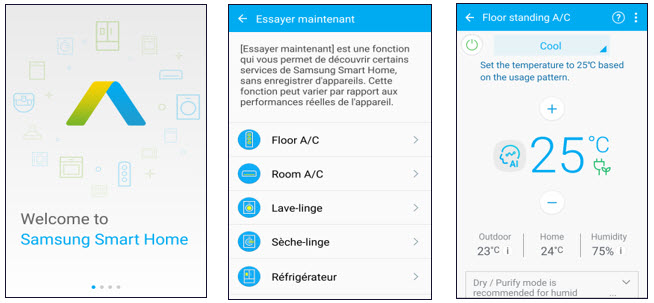
\includegraphics[scale=0.9]{samsung.jpg}
\caption{L'application Samsung Smart Home}
\label{fig:fig1}
\end{figure}
Avec plus de 1 million de téléchargements recensés à ce jour, l’application « Samsung Smart Home » est une référence en terme d’application de domotique et IOT.
Cette application permet aux utilisateurs de se connecter facilement avec divers appareils ménagers, y compris le réfrigérateur, machine à laver, climatiseur, four, aspirateur à vide et plus à travers vos smartphones permettant de surveiller et contrôler les appareils électroménagers Samsung sur la route et profiter des services utiles, y compris vérification de l'état, le contrôle de l'appareil, vue sur la maison, et le soutien à la clientèle.\\
Par contre, on remarque l’absence de quelque service comme :
\begin{itemize}
\item La possibilité de contrôler l’arrosage du jardin grâce à un système d’arrosage automatique communiquant directement avec son smartphone ou son PC.
\item La possibilité de contrôler les lampes et les volets pour plus de confort et une bonne gestion de l’énergie de la maison.
\item La possibilité de mieux renforcer son système de sécurité dans le cas d’un intrus ou d’un incendie et même une fuite de gaz avec un système d’alarme plus propice et plus évolué.
\end{itemize}


\section{Analyse Préalable}
On a commencé par une étude de faisabilité du projet d'une manière globale et simple qui centre sur les besoins des utilisateurs du système. En effet, avant de commencer l’étude préalable, il faut bien comprendre le système et ses intérêts.
On a commencé par une étude de faisabilité du projet d'une manière globale et simple qui centre sur les besoins des utilisateurs du système. En effet, avant de commencer l’étude préalable, il faut bien comprendre le système et ses intérêts. \\
\textbf{C’est quoi exactement ? } \\
La domotique c'est l'informatique appliquée à l'ensemble des systèmes de régulation, de gestion, de communication et de sécurité concernant l'habitat et les tâches de la vie quotidienne. \\
\textbf{Quel est son but ?} \\
La domotique permet d'améliorer le Confort, la Sécurité et la Fonctionnalité de l'habitat. \\
\textbf{Quand intervient-elle ?} \\
Lors de l'utilisation d'appareils électriques. \\
\textbf{Qui peut en avoir besoin ?} \\
La domotique s'adresse au simple bricoleur ainsi qu'à toute personne ayant besoin d'automatisation dans la maison (pour les handicapés par exemple) \\
\textbf{Où pouvons-nous l’utiliser ? } \\
On peut l'utiliser dans l'habitat.\\
\textbf{Comment ça fonctionne ? } \\
La domotique est basée sur la mise en réseau des différents appareils électriques de la maison. Les informations passent par le réseau électrique. \\

\bigskip

\section{Analyse des Besoins}

\subsection{Besoins Non Fonctionnels}
\begin{itemize}
    \item \textbf{Matériel} : Le système doit être compatible à la maison dans laquelle le système va être implémenté. Ainsi, l’application reliée à ce système doit être supporté par les appareils de l’utilisateur.
    \item \textbf{La Confidentialité} : L’authentification se fait par l’administrateur qui peut changer les paramètres par défaut en entrant son pseudo et son mot de passe. D’autre part on trouve un autre mode qui ne nécessite pas l’authentification qui est utilisé, par exemple, par les enfants dont le but de ne pas toucher les paramètres par défaut.
    \item \textbf{La Simplicité} : Le système doit être simple à utiliser, offrant des interfaces qui facilitent l’accès et la modification des paramètres et impressionnantes à voir.
Comportements en cas de panne : Le système est doté d'un utilitaire de détection de panne ainsi qu'une éventuelle correction. Pour les pannes persistantes, les appareils visent à informer l'utilisateur des erreurs produites en lui cédant des alertes.

    \item \textbf{Sécurité} : Le système doit crypter tous les données enregistrés, et doit avoir un par-feu pour interdir les périphériques inconnus à se connecter.
    
    \item \textbf{Prix} : Il comprend le coût de l’installation électrique, des logiciels de supervision et de l’intervention d’un expert pour la configuration et l’adaptation du système.
    \item \textbf{Facilité de déploiment} : La configuration doit être accessible à des personnes non-expertes en domotique pour adapter le système à l’utilisateur dépendant dont les besoins peuvent évoluer rapidement.
    
    \item \textbf{Évolutivité} : Des nouveaux protocoles de “haut niveau” doivent pouvoir être intégrés sans avoir à modifier le travail de conception initial selon la demande du client.
Notre futur objectif : est de veiller sur les personnes ayant des handicaps moteurs, visuels auditifs ou cognitifs ainsi que sur les personnes âgées, dans le cadre du maintien à domicile.
\end{itemize}

\subsection{Besoins Fonctionnels}
Le système domotique offre des diverses fonctionnalités à l’utilisateur pour lui assurer la sécurité, la flexibilité et le confort. \\

\begin{itemize}

\item \textbf{Contrôle du bâtiment, supervision :} 
Visualiser et exploiter votre bâtiment en temps réel, afin de piloter toutes les installations techniques, de faire face aux besoins énergétiques, d’établir une maintenance préventive.

\item \textbf{Gestion des consommations énergétiques :}
Mesurer et enregistrer tous les consommations électriques, thermique, hydraulique, garder la maîtrise des ressources et des contrats.

\item \textbf{Gestion des apports naturels, Façade bioclimatique et dynamique :}
Automatiser les stores en fonction des conditions climatiques, afin optimiser la lumière du jour et contrôler les échanges thermiques. 

\item \textbf{Contrôle des éclairages, Mise en valeur du bâtiment :}
Une régulation active permet d’économiser de 20 \% à 60 \% de l’électricité utilisée pour l’éclairage, en fonction de la saison, de la météo et de l’implantation du bâtiment.

\item \textbf{Régulation et Optimisation de la température :}
En fonction de l’occupation, de l’activité et des conditions climatiques, un contrôle total des équipements de Chauffage, de ventilation et de climatisation.

\item \textbf{Mesures thermiques et climatiques :}
Prise en charges des données météo, de la structure et de l’inertie du bâtiment pour anticiper les besoins et optimiser le confort thermique. 


\item \textbf{Contrôle et visualisation des installations :}
Surveiller la disponibilité de vos installations, être informé en local ou à distance, ajuster au juste besoin vos consignes, vos programmes horaires.
\end{itemize}




\section*{Conclusion}
L'objectif de cette partie était de présenter les fondements théoriques du projet en se basant en premièr lieux sur l'étude des applications similaires existants sur le marché, et dans un deuxième lieux sur un analyse des besoins fonctionnels et non fonctionnels de notre application.


%==============================================================================
\end{spacing}
